\chapter{Introduction}
\label{ch:Introduction}

% what are we trying to solve / what is the problem?
% why is it important?

% minimize faulty material
% change contact pressure of steel belt rolls if something's going wrong
% cost reduction
% automatization (IoT, Industry 4.0)

% perform quality checks with sensors
% mechanical parameters can be calculated from magnetic field data
% highly sensitive MEMS gradient magnetometer
% try to predict faulty material in real time

Industry is ever-changing. Especially people working in the information technology branch know that. The rise of the so-called Industry 4.0 is the perfect example. This means that mechanical processes are combined with modern information- communication technology.

Industry 4.0 is a term that was coined by Germany's research-union. It describes the fourth industrial revolution. As many people know the first industrial revolution took place with the rise of water- and steam-powered machines, the second revolution happened with the introduction of labour division and mass production. The third industrial revolution occured with the invention of computers, robots and computer automation. The fourth and final one basically just refines the third revolution. This revolution includes the term "cyper-physical systems", which are systems that are controlled by computers, algorithms and sensors. This also means that there has to be some kind of communication between these systems which happens mostly over the internet. Figure \ref{fig:industry40} depicts this sequence of revolutions.

\begin{figure}[H]
    \centering
    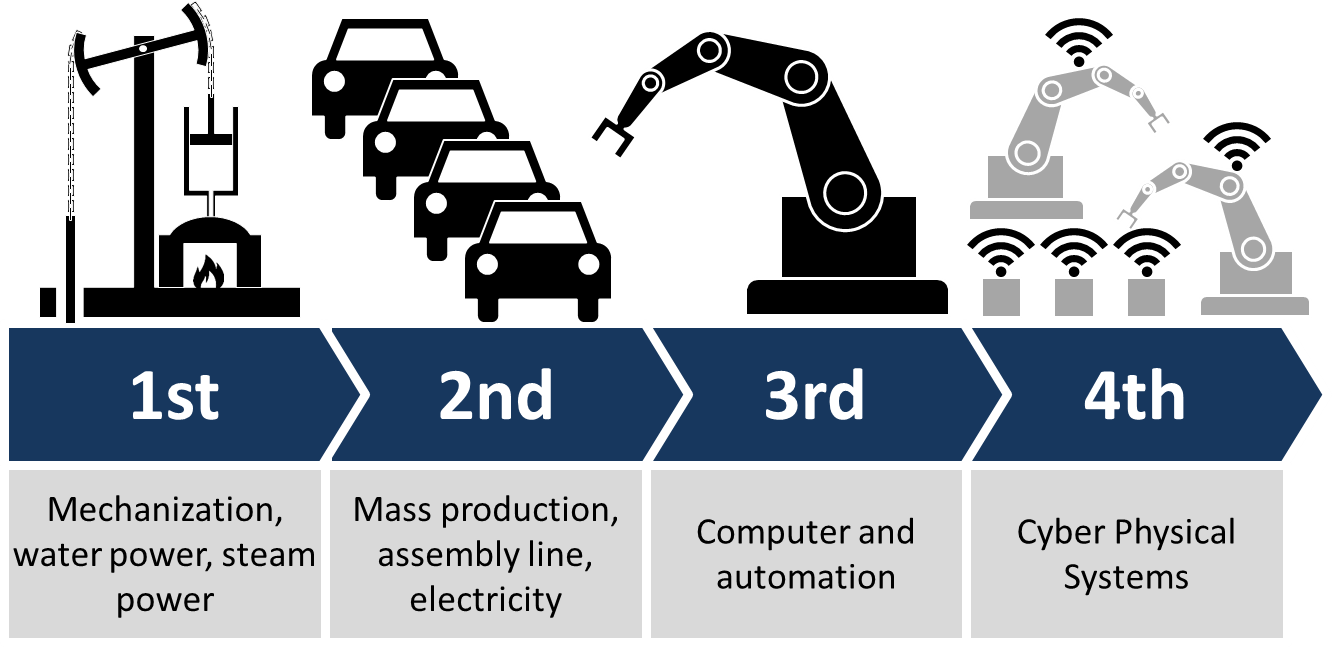
\includegraphics[width=11cm,keepaspectratio]{industry40}
    \caption{The four industrial revolutions that took place over the last centuries. \cite{img:industry4.0}}
    \label{fig:industry40}
\end{figure}

\section{Task}

The task of this diploma-thesis is to develop a system to read data from a sensor, process it and visualize it from a highly sensitive MEMS gradient magnetometer. This process should be as close to real-time as possible. This system should also be able to predict parameters of the measured material on the basis of the available data.

The specification of GRAMOC was defined together with the client as follows:

\begin{itemize}
    \item Receive sensor data from the sensor over UDP
    \item Save the data to HDF5 files for further processing
    \item Calculate regression parameters from the data
    \item Send the data and additional information to connected clients
    \item Visualize the received data
\end{itemize}

\section{Current Solutions}

% continuous quality inspection of steel belts
% current solution:
%   produce a certain amount
%   take sample
%   use sample to perform quality checks (stretch tests, ...)
% waste of material / low yield
% time consuming
% not automatable

% real time plotting
% a lot of solutions exist
% little solutions transfer data over network, many assume that sensor is attached to computer
% also no big data volume

\section{Outline}

% OUTLINE
% short summary of thesis
% explain two phases (I & II)
%   first phase => experimental, learning by doing
%   second phase => 'we know what we were doing', better planned


